\section{Results}\label{sec:results}

\subsection{The headline lift and its non-transfer}\label{results:headline}

The adapter lifts cold multiple-choice scoring substantially (\cref{tab:headline}:
ARC $+35.0$, TruthfulQA mc1 $+37.25$; transfer benchmarks HellaSwag $+17.0$,
Winogrande $+19.0$) and loses on generation in every condition (\cref{tab:genface}:
gsm8k loss, canonical magnitude $\mathbf{-25\pp}$ per R6 --- flat across a
generation-budget sweep, so a mechanistic multi-step-reasoning breakage, not
truncation). The generation loss that anchors the trade is gsm8k, which is verified
and canonical (the R6probe/L3 per-run forensic on the v7mc arm: 295/400 correct, 79
clean-wrong with a normal-terminating wrong \code{\#\#\#\#} numeral, 26
non-terminating reasoning loops, 0 empties) and R6-confirmed; lambada ($-32$) was an
\emph{illustrative} custom-token-norm scorer and the lm-eval confirmation (R9,
\code{lambada\_\allowbreak openai} template-off) is \textbf{not yet run}, so we do not count it
among the verified headline losses (\cref{tab:genface}). The scoring lift and the
generation loss are the two halves the rest of the paper reconciles.

The lift is not an artifact of the zero-shot floor, but the anti-floor control
resolves into \emph{two} distinct quantities and we report both rather than let one
stand in for the other. A paired 5-shot control (pre-registered eval R2, same
$n{=}400$) raises the base itself --- ARC $0.505{\rightarrow}0.635$, HellaSwag
$0.540{\rightarrow}0.610$, Winogrande $0.6575{\rightarrow}0.765$ --- closing
\textbf{37\% of the ARC headline, 41\% of HellaSwag's, and 57\% of Winogrande's}.
Against that better-prompted base, the \textbf{anti-floor} quantity (a@0 $-$ b@5:
the zero-shot adapter against a base given every prompting advantage, which is what
the kill-rule asks) is ARC $\mathbf{+22.0\pp}$, HellaSwag $\mathbf{+10.0\pp}$,
Winogrande $\mathbf{+8.25\pp}$. The \textbf{matched-shot} quantity (a@5 $-$ b@5:
whether the adapter still wins when few-shot is granted to both arms) is ARC
$\mathbf{+22.25\pp}$ (acc\_norm, paired McNemar over base-wrong items: 99 fixed vs
10 broken, $p{\approx}10^{-19}$), HellaSwag $\mathbf{+17.5\pp}$, Winogrande
$\mathbf{+13.75\pp}$. On ARC the two nearly coincide ($+22.0$ vs $+22.25$) because
the adapter is already saturated there (v7mc@5 ${\approx}$ v7mc@0); on Winogrande
they diverge sharply ($+8.25$ vs $+13.75$), and the anti-floor figure is the one we
treat as the bound. Per-item on ARC (198 base-wrong at 0-shot), the adapter fixes
151 (76.3\%) against few-shot's 69 (34.8\%) and covers $64/69 = \mathbf{92.8\%}$ of
the few-shot-fixed items (87 only-adapter, 5 only-few-shot); saturation is
task-specific --- v7mc@5 ${\approx}$ v7mc@0 on ARC (0.8575 vs 0.855) and TruthfulQA
(0.81 vs 0.810), while few-shot still stacks on the adapter for HellaSwag
($0.785 > 0.710$) and Winogrande ($0.9025 > 0.8475$). The headline remains the
zero-shot $+35.0$, and the anti-floor bound on it is $\mathbf{+22.0}$.

The lift is also protocol-bound in a second, sharper sense: with the chat template
removed entirely (R1b, same $n{=}400$ harness), \emph{both} arms collapse to
near-chance on ARC (base acc\_norm 0.25, adapter 0.285) --- there is no lift to
exploit outside the chat-template readout. This is direct evidence that the object
of study is the readout protocol itself, and it scopes every claim in this paper to
cold-MC scoring under a chat template.

The TruthfulQA $+37.25$ is reported separately and carries \textbf{no} anti-floor
control (the lm-eval \code{truthfulqa\_\allowbreak mc1} task fixes num\_fewshot=0, so both arms
ran 0-shot in R2); only ARC/HellaSwag/Winogrande have a real 5-shot control. We
further scope the $+37.25$ as a \textbf{selection lift on the mc1 metric}
(paired-significant, Holm-corrected $p_{\mathrm{corr}}$ $6.26\times10^{-38}$),
\textbf{not} a truthfulness gain and never as evidence for the off-axis mechanism
(it is largely answer-prior, \cref{disc:heterogeneity}).

The held-out-plus-mc2 control has now \textbf{run} (full set $n{=}817$): the lift
\textbf{generalizes held-out} ($\Delta_{\mathrm{UNSEEN}}$ mc1
$+37.8 \approx \Delta_{\mathrm{SEEN}}$ $+36.9$; mc2 $\Delta_{\mathrm{UNSEEN}}$
$+26.1$), so it is real beyond the mc1 selection metric and is \textbf{not}
memorization (the matched train covers ${\sim}79.9\%$ of the eval, yet the held-out
gain is undiminished), whereas a generic Align control collapses held-out (mc1
$+7.9$), marking the contrastive lift as the genuine, generalizing one. We therefore
report it as a real, held-out, generalizing \textbf{answer-prior} lift on mc1/mc2
(\cref{disc:heterogeneity}) --- never as truthfulness and never as the off-axis
mechanism.

\subsection{The fixed items are CoT-reachable --- an upper bound on
knowledge-accessibility}\label{results:arbiter}

The non-transfer is not a failure to teach the model anything; it is that the model
already knew. Of the 124 ARC items the adapter fixes in cold scoring (and the
on-axis offset does not), the base solves $124/124$ ($1.000$) under generative
chain-of-thought --- the rate of the items it already scores correctly cold
(base-right control, $200/202 = 0.990$) --- so the fixed items are knowledge the
base reaches by reasoning but that cold scoring misranks (\cref{tab:arbiter}). A
negative control decides whether that number discriminates or merely restates a
ceiling, and it is available from the same run: on the adapter's \textbf{residual}
--- the 47 items that are base-wrong and that the adapter does \emph{not} fix ---
base CoT accuracy falls to $\mathbf{41/47 = 0.872}$ (CI $[0.748, 0.940]$), against
$151/151$ on the base-wrong items it \emph{does} fix (Fisher
$p=1.4\times10^{-4}$) and $392/400 = 0.980$ over all of ARC ($p=0.0015$). The
arbiter therefore carries information about which items the adapter moves. We attach
the magnitude caveat rather than oversell it: ARC sits near its CoT ceiling in every
population, so the contrast is statistically clear but absolutely modest, and the
residual figure landed between the two thresholds we pre-registered for this control
(${\leq}0.85$ ``discriminates'' / ${\approx}0.97$ ``saturated'') --- we read it as
discriminating on the strength of the contrast, not of the point estimate. We read
the 124/124 as an \emph{upper bound} on knowledge-accessibility, not a proof of
perfect recall: it is a greedy $k{=}1$ arbiter, and for HellaSwag/Winogrande it runs
in a letter-MCQ format distinct from the cold-MC channel (\cref{method:protocol}).
Its robustness is corroborated independently: base self-consistency CoT at $k{=}3$
also reaches 124/124 on this set (\cref{sec:open}), so the result is not an artifact
of the single greedy chain. This holds out-of-task too: on GPQA the base solves the
items under chain-of-thought at $0.7071$ (arbiter), well above chance, so there is
no generative headroom a scoring shortcut could supply, and we therefore did not
build a verifier-guided arm (a design choice following from the no-headroom result,
not an independent test). And measured directly, the cold-MC lift on GPQA is itself
${\sim}0$ (base $0.4747 \rightarrow$ adapter $0.4697$, $-0.5\pp$, CI crossing zero):
the no-transfer is confirmed out-of-task (GPQA is out-of-task and
distribution-distant --- it is also the B.2 spillover task at $-6.6\pp$ --- so this
is a no-transfer-out-of-task result, not a no-transfer-to-hard one;
\cref{disc:arbiter} separates difficulty from distribution with within-format and
second-anchor controls). The adapter is not inert there --- it fixes ${\sim}21$ of
104 base-wrong items at a 0.202 fix-rate and breaks ${\sim}22$ base-right ones for a
net of about $-1$ --- but that exchange is churn within noise (no McNemar test), not
compensatory damage. Note the converse implication we do not hide: GPQA leaves
${\sim}23\pp$ of cold-scoring headroom (cold 0.4747 vs CoT 0.7071) that the adapter
fails to recover --- the adapter is not a general repair of the lossy readout but an
in-distribution exploit of it, which is exactly what the off-axis-of-degree geometry
predicts.

\subsection{Much of the lift is inducible without the contrastive objective, and how
much depends on capacity and on the task}\label{results:generic}

Two non-contrastive controls bound how much of the lift the \emph{objective} is
responsible for, and they answer different questions because they sit at opposite
ends of the capacity range (\cref{tab:inducibility}).

\textbf{At identical capacity.} A \emph{same-parameterization} control --- the
identical 48 head-pairs and identical $12{,}336$ trainable parameters as the adapter,
the same corpus, steps, split and checkpoint rule, with ordinary cross-entropy on the
correct answer and \emph{no} term against the incorrect one, three seeds --- recovers
$\mathbf{36.2\% \pm 5.0}$ of the ARC lift (best-checkpoint; $39.7\% \pm 3.1$ at the
fixed final step, so ${\sim}36$--$40\%$ is the honest range). This is the control that
isolates the objective, because the intervention space is held exactly fixed.

\textbf{At much higher capacity.} A non-contrastive Align-LoRA --- data- and
step-matched but with $1{,}800\times$ to $58{,}000\times$ more trainable parameters
(\cref{sec:definitions}) --- recovers ${\sim}62\%$, flat across a rank sweep
(59/63/60/65; slope-CI $[-1.4, +3.4]$ includes zero) and not raised by a best-effort
r512 flank (frac $0.22$ at lr1e-4, converged but overfitting; below-base at lr2e-4).

So the fraction a generic objective recovers is \emph{not} a single constant: it moves
from ${\sim}37\%$ at the adapter's own capacity to ${\sim}62\%$ with three-to-five
orders of magnitude more parameters. We therefore report inducibility as a
capacity-dependent quantity rather than as one number, and we do not claim a ceiling
for generic fine-tuning: within the grids we tested, more capacity buys more recovery.

\textbf{It is also strongly task-dependent} --- the same three same-parameterization
seeds recover $\mathbf{79.5\% \pm 1.4}$ of the Winogrande lift and
$\mathbf{69.5\% \pm 6.4}$ of HellaSwag's, but $\mathbf{0.9\% \pm 3.3}$ of
TruthfulQA-mc1's, i.e.\ nothing, even though TruthfulQA is in the control's own
training corpus (\cref{tab:inducibility}). The pattern is legible: where the task is
scored by the plausibility of a continuation (Winogrande, HellaSwag) simply raising
the log-probability of the correct option induces most of the lift, whereas where the
task requires \emph{beating a plausible distractor} --- which is precisely what
TruthfulQA-mc1 is built to test --- the contrastive term is doing work that ordinary
cross-entropy does not. ARC sits between the two. ``Most of the lift is generic'' is
therefore true of Winogrande and HellaSwag, and of ARC only at high capacity; it is
false at matched capacity on ARC and false throughout on TruthfulQA. TruthfulQA is
in any case excluded from the higher-capacity control as train-on-eval leakage
(held-out, the highest-rank control collapses $92\%{\rightarrow}30\%$).

\textbf{This ordering is a metric statement, and we say so here rather than only in
\cref{lim:metric}.} The inducibility fractions are computed on the same per-task
metric as the headline lifts, which for HellaSwag is acc\_norm. Recomputed on raw
accuracy the ordering does not survive: HellaSwag's $69.5\%$ becomes $8.9\%$ for this
control and $92.6\%$ becomes $19.1\%$ for the higher-capacity arm, while ARC's
same-parameterization $36.2\%$ becomes $26.9\%$ in Gemma and $27.2\%$ becomes
$59.7\%$ in Qwen. The four \emph{lifts} are robust to the choice; the cross-task
\emph{ordering} of inducibility is not, and no mechanistic claim in this paper rests
on it.

% ------------------------------------------------------------------ Table 1
\begin{table}[tbp]
\centering
\begin{threeparttable}
\caption{\textbf{Headline scoring-face MC lift} (V7-mc, Gemma~4 31B IT, $n{=}400$,
chat-template, lm-eval canonical). The cold-scoring lift the whole paper is about.
Same flags both arms; never cited without the gen-face row (\cref{tab:genface}) and
the protocol caveat (base ${\approx}0.50$ is loglik-MC scoring-face, \emph{not} a
third-party-reported ${\sim}91\%$ gen-CoT figure --- a blog, not Google's official
technical report). TruthfulQA-mc1 is reported separately as an answer-prior
selection lift (mechanism-excluded; it generalizes held-out ---
\cref{tab:heterogeneity}), never as a truthfulness gain and never as evidence for
the off-axis mechanism.}
\label{tab:headline}
\small
\begin{tabular}{lcccl}
\toprule
Benchmark & Base & V7-mc & Lift & Source artifact \\
\midrule
ARC-Challenge (acc\_norm) & 0.505 & 0.855 & $\mathbf{+35.0}$ &
  \code{msap-\allowbreak a1-\allowbreak trio-\allowbreak b2-\allowbreak planner-\allowbreak 2026-\allowbreak 06-\allowbreak 10} \\
TruthfulQA-mc1 & 0.4375 & 0.810 & $\mathbf{+37.25}$ & same \\
HellaSwag (acc\_norm) & 0.540 & 0.710 & $\mathbf{+17.0}$ & same \\
Winogrande & 0.6575 & 0.8475 & $\mathbf{+19.0}$ & same \\
\bottomrule
\end{tabular}
\begin{tablenotes}[flushleft]\footnotesize
\item Pre-registered with kill-rules; the anti-floor kill-rule \textbf{R2 has
executed ($n{=}400$) and the lift survived}. The paired 5-shot control, its two
named quantities (\textbf{anti-floor} a@0 $-$ b@5: ARC $\mathbf{+22.0\pp}$ / HSwag
$\mathbf{+10.0\pp}$ / Wino $\mathbf{+8.25\pp}$; \textbf{matched-shot} a@5 $-$ b@5:
ARC $\mathbf{+22.25\pp}$, McNemar b=99/c=10, $p{\approx}10^{-19}$ / HSwag
$\mathbf{+17.5\pp}$ / Wino $\mathbf{+13.75\pp}$; few-shot closes 37/41/57\% of the
respective headlines), the per-item coverage, and the task-specific saturation are
reported in \cref{results:headline}. \textbf{TQA carries no anti-floor control}
(lm-eval \code{truthfulqa\_\allowbreak mc1} fixes num\_fewshot=0; both arms 0-shot)
$\rightarrow$ cite the $+37.25$ separately, with no ``irreducible-to-few-shot''
claim. The artifact-backed replication is verified.
\item \textbf{Paired significance ($n{=}400$).} All four lifts are
\textbf{paired-significant} by an exact McNemar test computed over byte-identical
base/adapter items (prompts byte-identical 400/400 per task, 0 truncation): ARC
b=11/c=151 $p=1.32\times10^{-32}$, TQA b=6/c=155 $p=1.57\times10^{-38}$, Winogrande
b=23/c=99 $p=1.99\times10^{-12}$, HellaSwag b=39/c=107 $p=1.63\times10^{-8}$. They
survive \textbf{Holm--Bonferroni} correction across the four anchors ($m{=}4$):
$p_{\mathrm{corr}}$ ARC $3.95\times10^{-32}$, TQA $6.26\times10^{-38}$, Wino
$3.98\times10^{-12}$, HSwag $1.63\times10^{-8}$ --- every anchor at or below
$1.63\times10^{-8}$, \textbf{none dropped}. \emph{Scope caveat:} this certifies the
effect \textbf{exists and is paired-significant}, not that it is on-axis --- the
on-axis ceiling is $\Wknow$ 6.4\% (\cref{disc:geometry}). \emph{Metric note:} the
headline mixes acc\_norm (ARC/HSwag) with acc (TQA/Wino, which define no acc\_norm);
on HSwag acc\_norm ${\leq}$ acc ($+17.0$ vs $+22.25$), so the length-normalized
headline is the conservative figure, not a length artifact.
\end{tablenotes}
\end{threeparttable}
\end{table}

% ------------------------------------------------------------------ Table 2
\begin{table}[tbp]
\centering
\begin{threeparttable}
\caption{\textbf{Gen-face: V7-mc loses on generation} (Gemma~4 31B IT). The other
half of the trade. The verified anchor is \textbf{gsm8k}, the direct ``ARC-in-CoT''
test (\code{generate\_\allowbreak until}, exact\_match on the generation): V7-mc loses in every
condition. \textbf{Direction (loss) is robust; the canonical magnitude is
$-25\pp$} (R6 kill-rule PASS: base 0.9775 vs v7mc 0.7275, apples-to-apples
template-ON 5-shot, flat across cap \{512, 2048\} $\rightarrow$ mechanistic
multi-step-reasoning breakage, not truncation). \textbf{Across three independently
trained adapters the loss is $-24.2 \pm 7.3\pp$} (range $-16.5$ to $-31$;
\cref{tab:seeds}): the \emph{sign} replicates in 3/3 seeds, the magnitude varies by
about a factor of two, so the $-25$ here is this run's value and near the middle of
the observed range rather than a constant of the method. The retrieval-side \textbf{lambada}
loss ($-32$) is reported here only as an \emph{illustrative} signal: it comes from a
custom token-norm scorer, and the lm-eval confirmation (R9, \code{lambada\_\allowbreak openai}
template-off) is not yet run, so the inference/retrieval trade-off in this paper
rests on gsm8k alone, not on lambada.}
\label{tab:genface}
\small
\begin{tabular}{L{4.5cm}cccL{4.6cm}}
\toprule
Benchmark & Base & V7-mc & $\Delta$ & Source artifact \\
\midrule
gsm8k (A1 run, strict-match) & 0.9775 & 0.7275 & $\mathbf{-25.0}$ & A1 run, lm-eval
canonical; confirmed R6 \\
gsm8k (day3, mu\_only) & ${\sim}0.955$ & 0.905 & $-5$ &
\code{runs/\allowbreak phase4\_\allowbreak routed/\allowbreak day3/\allowbreak } \\
gsm8k (day3, romulo) & ${\sim}0.955$ & 0.785 & $-17$ & same \\
gsm8k (v7.5-baked, custom eval, $n{=}200$) & 0.955 & 0.17 & $\mathbf{-78}$ &
\code{runs/\allowbreak v7\_\allowbreak 5\_\allowbreak lofit/\allowbreak eval\_\allowbreak gsm8k\_\allowbreak v75.\allowbreak json} \\
\textbf{gsm8k canonical magnitude} & 0.9775 & 0.7275 & $\mathbf{-25.0}$ & R6
($n{=}400$ paired, apples-to-apples template-ON 5-shot, cap sweep
\{512, 2048\}=0.7275; template-OFF worse: base 0.730/v7mc 0.035, $-69\pp$; R6probe
agreed $-24\pp$) \\
lambada (illustrative) & 0.64 & 0.32 & $-32$ (ppl $11.6{\rightarrow}2523$) &
\code{runs/\allowbreak v7\_\allowbreak lofit\_\allowbreak gemma4\_\allowbreak 31b\_\allowbreak chat/\allowbreak eval/\allowbreak } --- \textbf{custom token-norm
scorer}, audit-verified 2026-06-10 \\
\bottomrule
\end{tabular}
\end{threeparttable}
\end{table}

% ------------------------------------------------------------------ Table 3
\begin{table}[tbp]
\centering
\begin{threeparttable}
\caption{\textbf{The fixed items are CoT-accessible; no transfer even on a hard
task (the per-item arbiter).} The core result. The adapter ``fixes'' items the base
already answers by reasoning; the gain is re-ranking, not capability --- and this
holds where the base must genuinely reason (GPQA).}
\label{tab:arbiter}
\footnotesize
\begin{tabular}{L{5.2cm} L{6.4cm} L{3.2cm}}
\toprule
Quantity & Value & Source artifact \\
\midrule
ARC items adapter fixes in cold MC but on-axis offset does not & 124 (mc\_only;
mc${\cap}$vinf=27 / mc\_only=124) &
\code{surface\_\allowbreak stratified\_\allowbreak arc\_\allowbreak challenge.\allowbreak json} \\
\addlinespace
Of those 124, base solves under generative CoT & $\mathbf{124/124 = 1.000}$
(fixed-parser re-run: n\_unparsed $5{\rightarrow}0$; the earlier ``123/124'' was a
parser artifact --- doc 128's numeric option label ``4'' the letter-parser could not
emit, now parses correct; ${\approx}$ base-right control 0.990) &
\code{arbiter\_\allowbreak arc\_\allowbreak cot\_\allowbreak v2.\allowbreak json} \\
\addlinespace
\textbf{Negative control --- adapter's residual} (base-wrong items it does
\emph{not} fix) & $\mathbf{41/47 = 0.872}$ CI$[0.748, 0.940]$ vs $\mathbf{151/151}$
on the ones it fixes (Fisher $\mathbf{p=1.4\times10^{-4}}$) and $392/400 = 0.980$
over all of ARC ($p=0.0015$) $\rightarrow$ \textbf{the arbiter discriminates};
robustness in the premise-file scaffold $66/73 = 0.904$ vs $326/327$
($p=3.6\times10^{-5}$). \emph{Same run, same protocol} (re-partition, no new
generation). Point estimate fell between the pre-registered ${\leq}0.85$ /
${\approx}0.97$ thresholds; reading rests on the contrast, and the absolute
magnitude is modest (ARC near its CoT ceiling throughout) &
\code{arbiter\_\allowbreak negative\_\allowbreak control\_\allowbreak b2.\allowbreak json}
(\code{analyze\_\allowbreak b2\_\allowbreak arbiter\_\allowbreak negative\_\allowbreak control.\allowbreak py}) \\
\addlinespace
Base-right control (already-correct-cold items) & $\mathbf{200/202 = 0.990}$
(fixed-parser run; the superseded pre-fix run gave $196/202 = 0.970$) &
\code{arbiter\_\allowbreak arc\_\allowbreak cot\_\allowbreak v2.\allowbreak json} \\
\addlinespace
Base GPQA accuracy under CoT (no-transfer is out-of-task, not difficulty-bound) &
$\mathbf{0.70}$ (139/198; thinking-ON greedy, max\_new=8192; thinking\_rate 1.000)
--- an earlier execution of the \emph{same} protocol; the per-item arbiter run scores
$140/198 = 0.7071$, differing by one item. The two share \code{build\_prompt},
\code{parse\_answer} and \code{build\_messages}, so this is the same apparatus
re-run, not independent corroboration &
\code{msap-\allowbreak phase1-\allowbreak 20260624} \code{b1\_\allowbreak gpqa\_\allowbreak base\_\allowbreak cot\_\allowbreak 8k.\allowbreak json} \\
\addlinespace
GPQA cold-MC scoring lift (adapter, out-of-task) & $\mathbf{-0.5\pp}$ (base 0.4747
$\rightarrow$ adapter 0.4697; CI crosses 0); arbiter base GPQA CoT 0.7071; fix-rate
0.202 over 104 base-wrong & \code{msap-\allowbreak phase1-\allowbreak 20260624} \\
\addlinespace
Reading & fixed items CoT-accessible; cold-MC misranks; no scoring headroom
out-of-task (GPQA lift ${\sim}0$) & --- \\
\bottomrule
\end{tabular}
\begin{tablenotes}[flushleft]\footnotesize
\item \textbf{GPQA note.} Base CoT $0.70 >$ chance $\rightarrow$ the base
\emph{does} reason these out, yet a scoring shortcut still cannot transfer
$\rightarrow$ the no-transfer is not an artifact of ARC being near its CoT ceiling.
We therefore did not build a verifier-guided arm (a design choice following from the
no-headroom result, not an independent test). With 2048 generation tokens the base
truncated 96\% of generations $\rightarrow$ a spurious 0.15; max\_new=8192 is
required. The GPQA figures are single-run (greedy) and directional (CI crosses 0),
not $n{=}400$-replicated like ARC.
\item \textbf{$0.7071$ is a floor.} $31/198$ traces ($15.7\%$) did not parse and are
scored as errors. The generations were not persisted --- the artifact stores only
\code{doc\_id}, correctness and the parsed letter --- so we cannot separate a
truncated chain from a malformed one without re-generating, and this project's own
rule is that truncation is decided by a token count and never by the parser. The
bias runs \emph{towards} the null we are arguing against: the true base CoT accuracy
is at least $0.7071$, so the ${\sim}23\pp$ of cold-to-CoT headroom quoted below is
conservative, and the claim that the base genuinely reasons GPQA out is if anything
understated. Re-generating with persisted traces is listed as future work.
\end{tablenotes}
\end{threeparttable}
\end{table}

% ------------------------------------------------------------------ Table 4 (3b)
\begin{table}[tbp]
\centering
\begin{threeparttable}
\caption{\textbf{How the readout misranks, and that the lift is not interpretable
re-scoring.} The \emph{how} of the readout failure (confident burial under fluency)
and the channel result (the lift does not reduce to re-scoring the output scalars).
All ARC-Challenge, Gemma~4 31B IT, base-wrong items unless noted.}
\label{tab:readout}
\footnotesize
\begin{tabular}{L{6.0cm} L{5.6cm} L{3.2cm}}
\toprule
Quantity & Value & Source artifact \\
\midrule
Base buries gold confidently --- chosen-vs-gold z-gap (adapter-independent
$S_{\mathrm{cot\_coldwrong}}$, $n{=}192$) & $\mathbf{1.45\sigma}$; gold-rank median
\textbf{2}; frac rank${\geq}2$ \textbf{0.59} &
\code{cold\_\allowbreak mc\_\allowbreak calibration\_\allowbreak arc\_\allowbreak challenge.\allowbreak json} \\
Consistency check ($S_{\mathrm{flip}}$, $n{=}151$, adapter-conditioned) & z-gap
$\mathbf{1.37\sigma}$; gold-rank median \textbf{2}; frac rank${\geq}2$ 0.54 & same \\
Gold-vs-distractor naive AUC (base-wrong, \emph{below} chance) & $\mathbf{0.394}$
CI$[0.356, 0.430]$, $n{=}204$ &
\code{residual\_\allowbreak discrimination\_\allowbreak arc\_\allowbreak challenge\_\allowbreak base.\allowbreak json} \\
Base raw pick = gold ($S_{\mathrm{cot\_coldwrong}}$ vs base-right control) &
$\mathbf{0.19}$ vs $\mathbf{0.81}$ & cold\_mc\_calibration \\
Entropy ``flatness'' is a softmax-temperature artifact & acc\_norm answer-entropy
0.920 ($S_{\mathrm{cot\_coldwrong}}$; length-norm compresses spread ${\sim}50\times$);
report rank/z-gap, not entropy & cold\_mc\_calibration \\
Adapter re-ranking is \textbf{promotion-dominated} ($S_{\mathrm{flip}}$) & gold-mass
$+0.35 >$ wrong-mass removed $+0.21$; $\Delta$entropy $-0.19$ &
cold\_mc\_calibration \code{re\_\allowbreak routing} \\
\textbf{Present-but-swamped:} PMI-residual AUC (same scalar channel, different
populations) & base-wrong $\mathbf{0.574}$ CI$[0.520, 0.627]$ $n{=}204$
\emph{(intermediate, CI\textsubscript{lo}${<}0.55$)} / adapter residual
$\mathbf{0.667}$ CI$[0.584, 0.744]$ $n{=}73$ \emph{(claim rests here)} &
\code{residual\_\allowbreak discrimination\_\allowbreak arc\_\allowbreak challenge\_\allowbreak \{base,mc\}.\allowbreak json} \\
\textbf{Surface ceiling} (supervised, held-out, base-wrong AUC) vs adapter &
logistic $\mathbf{0.458}$ / GBM $\mathbf{0.462}$ / on-test oracle stack
$\mathbf{0.502}$ (19\% recovery) / PMI $\mathbf{0.574}$ vs adapter $\mathbf{0.830}$
& \code{offaxis\_\allowbreak vs\_\allowbreak stack\_\allowbreak } +
\code{supervised\_\allowbreak surface\_\allowbreak ceiling\_\allowbreak arc\_\allowbreak challenge.\allowbreak json} \\
PMI applied to the adapter / adapter re-rank explained by surface & PMI
\textbf{hurts} $0.818{\rightarrow}0.758$; $R^2$(re-rank$\mid$surface)
$\mathbf{0.024}$ & \code{offaxis\_\allowbreak vs\_\allowbreak stack\_\allowbreak arc\_\allowbreak challenge.\allowbreak json} \\
\bottomrule
\end{tabular}
\begin{tablenotes}[flushleft]\footnotesize
\item \textbf{Reading.} The cold readout buries the gold under fluent surface forms
(z-gap $1.45\sigma$, naive AUC 0.394 \emph{below} chance), the correctness signal is
\emph{present but swamped} (PMI-residual clears chance on the adapter arm 0.667
$n{=}73$; base 0.574 $n{=}204$ intermediate --- \textbf{lossy, not empty}), and no
interpretable re-scoring of the output scalars recovers the lift (ceiling 0.574
${\ll}$ adapter 0.830; PMI \emph{hurts}; $R^2$ 0.024). The 0.830-vs-ceiling gap is
\textbf{information-set-confounded} (activations vs collapsed scalars) $\rightarrow$
a \textbf{channel} claim, not a ``magic direction'' (generic SFT recovers
${\sim}62\%$ the same way) nor ``empty channel''. \textbf{The in-space
activation-probe has now run and resolves this gate:} a logistic probe on the
\emph{same} per-head \code{o\_\allowbreak proj}-input activations (held out by item, same
cold-MC option-continuation distribution, preprocessing fit inside each fold,
within-item permutation null) recovers gold-vs-distractor on ARC base-wrong at
\textbf{AUC 0.955} CI$[0.934, 0.973]$ (null 0.494), against the \textbf{0.502}
collapsed-output surface-cap; a surface-form control on the option string caps at
\textbf{0.442} (${\approx}$ chance) $\rightarrow$ the 0.955 reads correctness the
output scalars discard, \textbf{not} a length/format artifact. This \textbf{widens
and cleans the channel gap ($0.502{\rightarrow}0.955$)} and supersedes the
preliminary wrong-space ${\sim}0.65$. \textbf{Three guards hold the read down to a
channel claim} (match \cref{disc:channel}): (1) the probe reads 12288 activation
dims while the adapter only nudges collapsed output logits --- different information
sets, so 0.955 is \textbf{not} ``probe beats adapter'' and \textbf{not} a
representational edit; (2) a linear probe decoding correctness ${\sim}0.95$ is
near-universal in capable LMs $\rightarrow$ it shows the info \emph{exists} in the
activations, \textbf{not} ``pure miscalibration / signal intact upstream'' --- we
keep \textbf{lossy} and drop ``pure miscalibration''; (3) the signal is
\textbf{diffuse} --- a random-48 head set decodes it at 0.949 CI$[0.924, 0.971]$
(null 0.492) ${\approx}$ the adapter's 48 heads $\rightarrow$ a \textbf{read-test}
that the cold-MC channel is lossy \emph{model-wide}, \textbf{decoupled} from the
\textbf{write-tests} that establish the adapter's specificity ($\Wknow$ 6.4\%,
random norm-matched \emph{offset} ${\sim}0\%$ recovery of the lift --- a different
operation; read ${\neq}$ write). TruthfulQA is \textbf{anchored out} of the channel
claim (probe 0.974 but surface-form control 0.639 + gold-first artifact 1.000
$\Rightarrow$ answer-prior, \cref{disc:heterogeneity}); the channel claim is
anchored on \textbf{ARC}.
\end{tablenotes}
\end{threeparttable}
\end{table}

% ------------------------------------------------------------------ Table 5 (4)
\begin{table}[tbp]
\centering
\begin{threeparttable}
\caption{\textbf{Inducibility is capacity- and task-dependent.} Two non-contrastive
controls. The \emph{same-parameterization} control holds the intervention space
exactly fixed (identical 48 head-pairs, identical $12{,}336$ parameters) and varies
only the objective, so it isolates the objective; the \emph{higher-capacity}
Align-LoRA is data- and step-matched but carries $1{,}800\times$--$58{,}000\times$
more parameters across the r8--r256 plateau ($117{,}000\times$ at the r512 flank). The fraction a generic objective recovers moves with both capacity
and task $\rightarrow$ the effect is \textbf{partly, not wholly, special to the
contrastive objective}. ARC is the clean test for the higher-capacity arm; TQA is
excluded there as train-on-eval leakage.}
\label{tab:inducibility}
\footnotesize
\begin{tabular}{L{5.4cm} L{6.6cm} L{2.8cm}}
\toprule
Quantity & Value & Source artifact \\
\midrule
\multicolumn{3}{l}{\emph{At identical capacity --- same-parameterization control
($12{,}336$ params, CE-plain, 3 seeds)}} \\
ARC lift recovered & fraction $\mathbf{36.2\% \pm 5.0}$ (best-ckpt; $39.7\% \pm 3.1$
final-ckpt) $\rightarrow$ honest range ${\sim}36$--$40\%$ &
\code{runs/\allowbreak e1\_\allowbreak plain\_\allowbreak ce/} \\
Task heterogeneity (same three seeds) & Winogrande $\mathbf{79.5\% \pm 1.4}$;
HellaSwag $\mathbf{69.5\% \pm 6.4}$; ARC $\mathbf{36.2\% \pm 5.0}$; TruthfulQA-mc1
$\mathbf{0.9\% \pm 3.3}$ (\emph{nothing}, despite TQA being in the control's own
training corpus) & same \\
\midrule
\multicolumn{3}{l}{\emph{At $1{,}800\times$--$58{,}000\times$ capacity ---
higher-capacity Align-LoRA}} \\
ARC lift recovered (rank sweep r8/32/64/256) & fraction
$\mathbf{59/63/60/65 = {\sim}62\%}$, flat & \code{msap-\allowbreak phase1-\allowbreak 20260624} (rank
sweep) \\
Within-sweep capacity slope & slope-CI $\mathbf{[-1.4, +3.4]}$ (includes
0); paired-bootstrap frac-CI $\mathbf{[51\%, 73\%]}$, delta-method
${\sim}[45\%, 85\%]$ (zone C, binned on the point) & same $+$ \code{l1\_\allowbreak paired\_\allowbreak bootstrap.\allowbreak json} \\
Best-effort capacity flank (r512, causal fairness, $n{=}400$) & lr1e-4 frac
$\mathbf{0.22}$ (converged, acc${>}$base; overfit ep2${\rightarrow}$ep4, robust
ep2=ep4); lr2e-4 \textbf{below base} (broken, excluded like r256hi) $\rightarrow$
\textbf{does not raise ${\sim}62\%$ within this grid} & \code{msap-\allowbreak align-\allowbreak fairness-\allowbreak 20260702} \\
TQA excluded --- leakage (proof) & frac 41/66/72/92 monotone${\uparrow}$; held-out
20\%: r256 $\mathbf{92\%{\rightarrow}30\%}$ (CI95 $[0.79, 1.06]$ on $n{=}400$
$\rightarrow$ $[0.05, 0.55]$ on the $n{=}82$ stratum, paired bootstrap; the
intervals do not overlap); the rank sweep flattens, r8=r256=0.524 on the full
$n{=}164$ held-out slice; contrastive generalizes held-out (0.83) &
\code{runs/\allowbreak align\_\allowbreak fairness/\allowbreak tqa\_\allowbreak heldout\_\allowbreak stratum\_\allowbreak ci.\allowbreak json} \\
\midrule
Residual not explained by the tested controls (ARC) & ${\sim}\mathbf{60}$--$\mathbf{64\%}$
at matched capacity; ${\sim}\mathbf{38\%}$ against the higher-capacity arm & derived \\
\bottomrule
\end{tabular}
\begin{tablenotes}[flushleft]\footnotesize
\item \textbf{Two r256 series, and which one the interval uses.} The rank-sweep row
above reports r256 at fraction $0.65$ (accuracy $0.7325$), taken from the
de-risking rank sweep; the paired-bootstrap interval $[51\%, 73\%]$ is computed on
the per-item canonical arm, where r256 reads accuracy $0.7225$ and fraction
$\mathbf{0.6214}$. These are different runs of the same configuration, not a
discrepancy in one: the sweep establishes flatness across ranks, the canonical arm
supplies the point and the interval, and the pre-specified zone binning is applied to
the canonical $0.6214$. Per-item files for r8/r32/r64 are not released, so the
\emph{slope} across ranks rests on the parametric sweep rather than on a per-item
re-derivation.
\item \textbf{The objective is non-contrastive; the selection rule is not.} The
same-parameterization arm's loss carries no term against the incorrect option, but
the checkpoint rule we inherited from the adapter validates on whether the correct
option outscores the incorrect one. It bit in one seed of three (seeds 1--2 select
the final step; seed 0 selects step 600 over 800), and there it picked the
\emph{worse} ARC checkpoint --- which is why the fixed-final variant, using no
validation signal at all, reads $39.7\% \pm 3.1$ against the $36.2\% \pm 5.0$ we
quote. The contamination deflates this control, so the contrastive-specific residual
is conservative. Provenance:
\code{runs/\allowbreak e1\_\allowbreak plain\_\allowbreak ce/\allowbreak offsets\_\allowbreak seed*.\allowbreak log.\allowbreak json}.
\item \textbf{Note.} We report these as the best observed recovery under the
generic-SFT family we tested, not as a bound on generic fine-tuning in general. Two
facts set the limits of the claim. (i) \emph{Capacity moves the fraction}: the same
non-contrastive objective recovers ${\sim}37\%$ at the adapter's own $12{,}336$
parameters and ${\sim}62\%$ with three-to-five orders of magnitude more, so no single
number is ``the'' generic fraction and we do not assert a ceiling. (ii) \emph{Within
each grid the fraction is flat}: the r8--r256 slope-CI includes zero and the r512
flank does not raise it (it recovers less at lr1e-4 and breaks below base at lr2e-4,
both excluded by the same convergence-pathology rule that excluded r256hi), so the
residual is not a gap that more rank closes \emph{within the tested rank/LR/epoch
grid}. What we cannot exclude is a different architecture, placement, optimizer or
search budget doing better.
\item \textbf{Interval validation and the r512 flank.} Because delta-method (Wald)
intervals on ratio estimators can be unstable when the denominator's sampling error
matters, the fraction interval is cross-checked twice. An independent
bootstrap-of-the-ratio (200k parametric draws from the published arm accuracies at
$n{=}400$, independent-binomial resampling) gives r256 frac CI
$[0.50, 0.80]$ against the delta-method $[0.45, 0.85]$, and a bootstrap slope CI of
$[-2.5, +4.6]$ pp per log2-rank step containing zero, both matching the published
reading (\code{runs/\allowbreak oq1\_\allowbreak functional\_\allowbreak axis/\allowbreak frac\_\allowbreak ci\_\allowbreak bootstrap.\allowbreak json}). That check was
conservative by construction --- resampling each arm independently discards the
correlation induced by scoring the \emph{same} $400$ items in all three arms --- and
we flagged that a paired design would only tighten it. It does: resampling items with
replacement and carrying base, generic and contrastive together (200k reps, seed $0$,
zero degenerate replicates) gives $\mathbf{[0.51, 0.73]}$, $44\%$ narrower than the
delta-method interval and contained in it, with the measured item-level correlation
($r{=}0.42$ base--generic, $0.26$ base--contrastive) as the mechanism. We report the
paired interval as primary and keep both others as conservative readings that contain
it (\code{...l1\_\allowbreak paired\_\allowbreak bootstrap.\allowbreak json}, superseding the independent-binomial
file above). The r512 flank
is deliberately \emph{not} folded into the flat-sweep fit: at lr 1e-4 it converges
yet recovers markedly less (0.22, stable across epochs 2--4, overfitting beyond),
and at lr 2e-4 it breaks below base --- both excluded by the same
convergence-pathology rule that excluded the r256 high-LR arm, so the flank
\emph{bounds} the sweep (more capacity does not raise the fraction) rather than
extending the regression.
\end{tablenotes}
\end{threeparttable}
\end{table}

% ------------------------------------------------------ Figure 1 + Table 6 (5)
\begin{figure}[t]
\centering
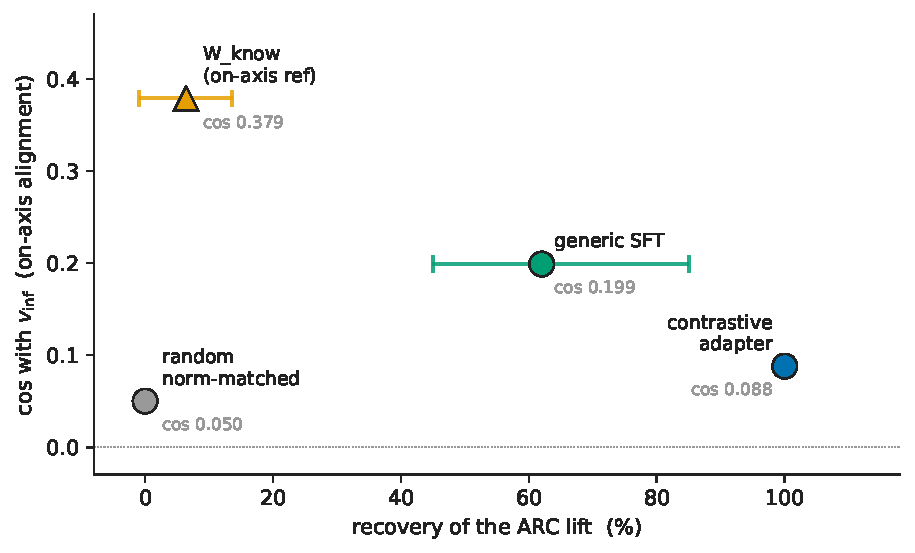
\includegraphics[width=\textwidth,alt={Scatter plot of the matched-control
spectrum: x-axis is the fraction of the ARC lift each direction recovers, y-axis is
the cosine with the functional correctness direction v_inf. Random floor near zero
recovery; the same-parameterization control near 37 percent at cosine 0.136;
higher-capacity generic SFT near 62 percent at cosine 0.199; the contrastive adapter
at 100 percent with the lowest cosine 0.094; and the on-axis reference W_know at high
cosine 0.379 but only 6.4 percent recovery.}]{figures/fig_geometry_spectrum.pdf}
\caption{\textbf{The matched-control spectrum on two independent axes.} $x$:
fraction of the ARC lift each direction recovers; $y$: cosine with the functional
correctness direction $\vinf$ (net effect on activations for the four methods; the
reference direction itself for $\Wknow$, marked $\blacktriangle$). The two orderings
are not monotone in each other: the most on-axis point ($\Wknow$, cos 0.379)
recovers only 6.4\%, while the top recoverer (the contrastive adapter, 100\%) is the
\emph{least} on-axis (cos 0.094). \textbf{The two non-contrastive controls separate
the two factors at work.} The \emph{same-parameterization} control (identical 48
head-pairs and $12{,}336$ parameters; only the objective differs) recovers
${\sim}37\%$ at cos $0.136$, while \emph{higher-capacity} generic SFT
($1{,}800\times$--$58{,}000\times$ more parameters) recovers ${\sim}62\%$ at cos
$0.199$: with the parameterization held fixed the contrastive objective is both
further off-axis and far more effective, whereas added capacity buys recovery while
moving \emph{toward} the axis. So how much a generic objective recovers depends on
capacity, and where the recovery lives depends on the objective --- two factors, not
one ordered scale. Horizontal bars are the published 95\% intervals on the recovery
fraction where one exists --- $\Wknow$ $[-0.9\%, +13.6\%]$ and generic SFT
$[51\%, 73\%]$ (paired bootstrap); the random floor (three seeds), the same-parameterization control
(three seeds, sd $5.0$ pp) and the contrastive anchor (100\% by construction) carry
none, and we do not synthesize one. \textbf{$\Wknow$'s interval crosses zero and
overlaps the random floor:} its 6.4\% is statistically indistinguishable from no
recovery (exact McNemar $p=0.136$), and it is counted with the floor rather than as a
rung. Values in \cref{tab:spectrum}.}
\label{fig:spectrum}
\end{figure}

\begin{table}[tbp]
\centering
\begin{threeparttable}
\caption{\textbf{Geometry spectrum: off-axis of degree, method-dependent.}
Apples-to-apples: the \emph{net effect on activations} of each method, decomposed
against the functional correctness direction $\vinf$. \code{ratio} = on-axis
alignment of the net effect with $\vinf$, normalized to a random direction (1.0 =
like random; higher = more on-axis than chance).}
\label{tab:spectrum}
\footnotesize
\begin{tabular}{L{3.2cm} L{6.2cm} L{2.8cm} L{2.6cm}}
\toprule
Direction & Recovery of the lift & cos with $\vinf$ (ratio vs chance) & Source
artifact \\
\midrule
random norm-matched (3 seeds) & $\mathbf{{\approx}0\%}$ (acc\_norm 0.50--0.52
${\approx}$ base 0.505) & 0.05 (1.0) & \code{msap-\allowbreak phase1-\allowbreak 20260624}
\code{derisk/\allowbreak offsets\_\allowbreak random\_\allowbreak s*} \\
on-axis maximum ($\Wknow$, Fisher-LDA) & $\mathbf{6.4\%}$ (ARC null 0.500 / mc
0.853 / wknow 0.522; \textbf{statistically indistinguishable from zero}: exact
McNemar b=10/c=19 $p=0.136$, paired-bootstrap frac-CI95 $[-0.009, +0.136]$ and
Wilson acc-CI $[0.474, 0.571]$ both include chance) & --- (cos with $\vinf$ 0.379;
cos with $\thetamc$ 0.0014) & \code{runs/\allowbreak wknow\_\allowbreak causal/\allowbreak } +
\code{msap-\allowbreak wknow-\allowbreak onaxis-\allowbreak 20260623} \\
contrastive adapter (net effect) & 100\% (by construction) & $\mathbf{0.088}$
\textbf{(1.74)}; across three seeds $0.094 \pm 0.008$ \textbf{($1.85 \pm 0.14$)};
direct $\thetamc$ offset cos 0.0014 & \code{msap-\allowbreak phase1-\allowbreak 20260624}
\code{derisk/\allowbreak contrastive\_\allowbreak direction}; \code{runs/\allowbreak v7\_\allowbreak lofit\_\allowbreak seed\{1,2\}/} \\
\textbf{same-parameterization control} (net effect, 3 seeds) --- \emph{same
intervention space, objective changed} & ${\sim}\mathbf{37\%}$ (ARC) &
$\mathbf{0.136 \pm 0.017}$ \textbf{($2.68 \pm 0.34$)} &
\code{runs/\allowbreak e1\_\allowbreak plain\_\allowbreak ce/\allowbreak neteffect\_\allowbreak seed*} \\
higher-capacity generic SFT (net effect) & ${\sim}\mathbf{62\%}$ & $\mathbf{0.199}$
\textbf{(3.93)} & \code{msap-\allowbreak phase1-\allowbreak 20260624} \code{derisk/\allowbreak align\_\allowbreak direction} \\
\bottomrule
\end{tabular}
\begin{tablenotes}[flushleft]\footnotesize
\item \textbf{Verdict.} All three methods are \textbf{mostly off-axis} (cos${<}0.2$,
${\sim}$78--85$^{\circ}$ from $\vinf$), but by different degrees, and the ordering is
informative: the contrastive adapter is the \emph{most} off-axis ($1.85$), the
same-parameterization control is intermediate ($2.68$), and higher-capacity generic
SFT is the least ($3.93$, $2.1\times$ more on-axis than the contrastive adapter)
$\rightarrow$ \textbf{off-axis of degree, not universal.}
\item \textbf{The same-parameterization arm is the load-bearing comparison here},
because it holds the intervention space exactly fixed (identical 48 head-pairs,
identical $12{,}336$ parameters) and changes \emph{only} the objective: with the
parameterization controlled, the contrastive objective lands
\textbf{further off-axis} ($1.85$ vs $2.68$) \emph{and} recovers substantially more
($100\%$ vs ${\sim}37\%$). The off-axis character is therefore not an artifact of the
LoFiT parameterization --- it tracks the objective.
\item \textbf{Two axes, not a ladder.} Recovery does not increase monotonically with
off-axis-ness: among the two \emph{non}-contrastive arms the more on-axis one
(higher-capacity SFT, $3.93$) recovers \emph{more} than the more off-axis one
(same-parameterization, $2.68$), because there capacity is the dominant variable. The
spectrum is organized by two factors --- objective and capacity --- and should not be
read as a single ordered scale.
\item The direct $\thetamc$ offset (cos 0.0014, a weight-space proxy) was misleading;
the clean net-activation-effect experiment is the canonical measurement.
\textbf{Forward filter:} a zero-cost read-space preview said ``off-axis'' (ratio
${\sim}1.05$); the clean experiment refuted it (3.93). Report only the clean
experiment.
\end{tablenotes}
\end{threeparttable}
\end{table}

% ------------------------------------------------------------------ Table 7 (6)
\begin{table}[tbp]
\centering
\begin{threeparttable}
\caption{\textbf{On-axis causal controls (no on-axis reference reproduces the
lift).} The earlier causal arms, consistent with \cref{tab:spectrum}'s spectrum:
pushing \emph{along} correctness does not recover the lift. (These on-axis causal
arms were measured on the vinf\_causal run, whose within-run MC baselines --- ARC
$+35.0$, TQA $+36.5$ --- differ slightly from the A1 canonical of
\cref{tab:headline}, $+37.25$; fractions are computed within-run.)}
\label{tab:onaxis}
\footnotesize
\begin{tabular}{L{5.4cm} L{6.6cm} L{2.8cm}}
\toprule
Quantity & Value & Source artifact \\
\midrule
ARC lift recovered by on-axis $\vinf$ (mass-mean, norm-matched) & fraction
$\mathbf{0.11}$ (MC $+35.0$ / VINF $+4.0$; $z = -6.63$, unpaired and conservative
--- the base stderr enters both lifts). \textbf{Paired over the same 400 items the
small recovery is detectable}: exact McNemar b=12/c=28 $p=0.017$, paired-bootstrap
frac-CI95 $[+0.027, +0.197]$ excludes 0. So the weaker on-axis reference recovers
\emph{little}, not \emph{nothing} --- unlike $\Wknow$ below &
\code{runs/\allowbreak vinf\_\allowbreak causal/\allowbreak vinf\_\allowbreak paired\_\allowbreak significance.\allowbreak json} +
\code{msap-\allowbreak vinf-\allowbreak causal-\allowbreak 20260623} \\
ARC lift recovered by $\Wknow$ (strongest on-axis ref) & fraction $\mathbf{0.064}$
(null 0.500 / mc 0.853 / wknow 0.522; ${\ll}$ 0.30 kill-rule;
\textbf{indistinguishable from zero}: exact McNemar b=10/c=19 $p=0.136$,
paired-bootstrap frac-CI95 $[-0.009, +0.136]$ includes 0) &
\code{runs/\allowbreak wknow\_\allowbreak causal/\allowbreak } \\
TQA lift recovered by either on-axis ref & $\mathbf{{\sim}0}$ (VINF $-2.75$;
$\Wknow$ ${\approx}$ null) & --- \\
$\thetamc$ vs $\vinf$ & $\coswh$ $\mathbf{-0.003}$ (within null); 6.4\% mass in top
PCs; norm $4.3\times$ class gap (the top-PC 6.4\% is coincidentally equal to the
$\Wknow$ recovery 6.4\%, not the same quantity) &
\code{theta\_\allowbreak mc\_\allowbreak character\allowbreak ization.\allowbreak json} \\
MMLU damage, on-axis $\vinf$ vs mc & VINF $-5.83$ ${\geq}$ MC $-4.30$ (gate PASS,
null MMLU $+0.07\pp$) & --- \\
\bottomrule
\end{tabular}
\begin{tablenotes}[flushleft]\footnotesize
\item \code{process-\allowbreak LoFiT-\allowbreak PRM} (an on-axis training program) is \textbf{refuted
causally} at eval time (a PRM corpus is not warranted); a \emph{training-time}
on-axis constraint \textbf{has now run and does not rescue transfer} (no $\lambda$
passes the lift-matched gate, so the $+35$ is the off-axis mass by
\emph{necessity}; see \cref{sec:open}).
\end{tablenotes}
\end{threeparttable}
\end{table}

% ------------------------------------------------------------------ Table 8 (7)
\begin{table}[tbp]
\centering
\begin{threeparttable}
\caption{\textbf{No layer locus: the lift scales with offset magnitude, not
layer.}}
\label{tab:locus}
\footnotesize
\begin{tabular}{L{5.6cm} L{6.6cm} L{2.6cm}}
\toprule
Quantity & Value & Source artifact \\
\midrule
corr(recovered lift, total offset magnitude $\Sigma|r|$) & $\mathbf{0.985}$ &
\code{msap-\allowbreak phase1-\allowbreak 20260624} \code{patch\_\allowbreak layers/\allowbreak *.\allowbreak json} \\
corr(recovered lift, head count) & 0.832 & same \\
``Layers 36--40 carry 87\%'' & head-count artifact (that band holds 71\% of adapter
heads); adapter spans L30--55 --- \textbf{not a causal locus} & same \\
\bottomrule
\end{tabular}
\end{threeparttable}
\end{table}

% ------------------------------------------------------------------ Table 9 (8)
\begin{table}[tbp]
\centering
\begin{threeparttable}
\caption{\textbf{Task heterogeneity: ARC ${\neq}$ TQA.} ARC is question-conditional
and carries the readout story; TQA is largely answer-prior / surface-form Goodhart.
The held-out + mc2 control has run: TQA generalizes held-out $\rightarrow$ reported
as a real, generalizing answer-prior lift, not as the off-axis mechanism.}
\label{tab:heterogeneity}
\footnotesize
\begin{tabular}{l L{3.6cm} L{6.2cm} L{2.8cm}}
\toprule
Task & Diagnostic & Value & Source artifact \\
\midrule
ARC & PMI-DC retention of lift & $\mathbf{78\%}$ (naive $+0.3275$ $\rightarrow$ PMI
$+0.2550$) & \code{pmi\_\allowbreak dc\_\allowbreak arc\_\allowbreak challenge.\allowbreak json} \\
ARC & choices-only lift & $\mathbf{+0.0375}$ CI$[-0.005, +0.08]$ (not clear) ---
question-conditional, not answer-prior &
\code{answer\_\allowbreak only\_\allowbreak arc\_\allowbreak challenge.\allowbreak json} \\
TQA & choices-only lift & $\mathbf{+0.2225}$ CI$[+0.1675, +0.2725]$ --- answer-prior
& \code{answer\_\allowbreak only\_\allowbreak truthfulqa\_\allowbreak mc1.\allowbreak json} \\
TQA & adapter picks correct option with NO question & $\mathbf{0.5725}$ (base 0.35,
chance 0.229) --- surface-form Goodhart
\citep{SurfaceFormCompetition,ChoicesOnlyCheater} & same \\
TQA & PMI-DC retention & 68\% & \code{pmi\_\allowbreak dc\_\allowbreak truthfulqa\_\allowbreak mc1.\allowbreak json} \\
TQA & paired significance of the $+37.25$ & exact McNemar b=6/c=155,
$p_{\mathrm{corr}}$ $\mathbf{6.26\times10^{-38}}$ (Holm $m{=}4$) & paired doc\_hash
400/400 \\
TQA & held-out generalization ${\neq}$ memorization (full set $n{=}817$; train
covers ${\sim}79.9\%$, 653 SEEN / 164 UNSEEN) & v7mc
$\mathbf{\Delta_{\mathrm{UNSEEN}}}$ \textbf{mc1} $\mathbf{+37.8}$ ${\approx}$
$\Delta_{\mathrm{SEEN}}$ $+36.9$; mc2 $\Delta_{\mathrm{UNSEEN}}$ $+26.1$ (gate
$\Delta_{\mathrm{UNSEEN}}$ mc1 ${\geq}+15$ AND $\Delta$mc2 ${>}+10$ passed); generic
Align \textbf{collapses held-out} (mc1 $+38.6{\rightarrow}\mathbf{+7.9}$; mc2
$+24.1{\rightarrow}+7.6$) & \code{analyze\_\allowbreak tqa\_\allowbreak contamination\_\allowbreak l4.\allowbreak py}, full 817 \\
\bottomrule
\end{tabular}
\begin{tablenotes}[flushleft]\footnotesize
\item \textbf{Note.} The lift is task-heterogeneous. TruthfulQA is an answer-prior
effect --- a generalizing selection lift on mc1/mc2 (the held-out + mc2 control
generalizes: $\Delta_{\mathrm{UNSEEN}}$ mc1 $+37.8$, so it is neither memorization
nor mc1-only, while a generic Align control collapses held-out to $+7.9$) --- but
it is not a truthfulness gain and not evidence for the off-axis mechanism. ARC is
question-conditional, off-axis-of-degree, and non-transferable.
\end{tablenotes}
\end{threeparttable}
\end{table}

% ------------------------------------------------------------------ Table 10 (9)
\begin{table}[tbp]
\centering
\begin{threeparttable}
\caption{\textbf{Deployment pathologies (coupled to injection method, not to the
lift).} The recovery introduces \textbf{two certified costs} --- no transfer to
generative CoT (multi-step reasoning breakage) and retrieval/recall spillover ---
that a generic SFT recovering most of the lift does not incur, so they trace to how
the contrastive offset is folded into weights, not to the lift itself. A third,
previously-listed cost --- an end-of-turn ``collapse'' --- is \textbf{retracted} as
a measurement artifact (last row). Rows 2--4 are \textbf{family} evidence from
sibling adapters (the D.1 SocialIQA and B.2/KR adapters), not the V7-mc adapter
under study; V7-mc's own directly-measured MMLU spillover is $\mathbf{-4.2\pp}$
(row 5).}
\label{tab:pathologies}
\footnotesize
\begin{tabular}{L{3.4cm} L{9.0cm} L{2.4cm}}
\toprule
Pathology & Value & Source artifact \\
\midrule
No-CoT-transfer (multi-step reasoning) & gsm8k loss every condition
(\cref{tab:genface}); contrastive baked ${\rightarrow}0.17$. \textbf{R6 canonical
(kill-rule PASS, apples-to-apples, template ON, 5-shot, $n{=}400$):} base
$\mathbf{0.9775}$ vs v7mc $\mathbf{0.7275}$ = $\mathbf{-25\pp}$, flat across cap
\{512, 2048\}=0.7275/0.7275 $\rightarrow$ \textbf{not truncation} (extra budget
never rescues; v7mc cap2048 runs ${\sim}$2h to the ceiling without improving;
template-OFF is worse --- base 0.730 / v7mc 0.035, $-69\pp$ --- so it is not a
template artifact). Forensic (R6probe @cap2048): 79 clean-wrong (\code{\#\#\#\#}
wrong number --- reasoning resolved but defective) + 26 degenerate non-terminating
loops already present @cap512 (the loop precedes the budget, not truncation).
\textbf{Align SFT preserves $0.96{\rightarrow}0.95$ (NS)} & R6
(\code{runs/\allowbreak mechanism\_\allowbreak v8/\allowbreak R6\_\allowbreak *}) + R6probe (\code{R6probe\_\allowbreak *}) +
\cref{tab:genface} \\
\addlinespace
Retrieval spillover (D.1 SocialIQA adapter --- family evidence) & MMLU
$\mathbf{-19.59\pp}$ ($0.8306{\rightarrow}0.6347$); K=12 not recovered ($-20.80$,
Pareto-worse) & D.1 SocialIQA spillover audit \\
Spillover (KR SciQ K=24) & GPQA Diamond $\mathbf{-12.1\pp}$ (sciq $+2.1\pp$
overshoot) & KR SciQ K=24 overshoot audit \\
Spillover (B.2 mc\_discrimination) & MMLU $-6.3\pp$ / GPQA $-6.6\pp$ & B.2 phase-3
findings \\
Spillover MMLU (V7-mc direct, eval-bulletproof R10) & $\mathbf{-4.2\pp}$
($0.8226{\rightarrow}0.7805$, ${\sim}$2k stratified, 0-shot) --- the V7-mc adapter
under study spillovers MMLU itself; same sign as B.2 ($-6.3\pp$), smaller &
\code{runs/\allowbreak eval\_\allowbreak bulletproof/\allowbreak R10\_\allowbreak *} \\
Spillover mechanism & $\coswh(\vinf, \vret)$ $\mathbf{+0.283}$
BCa95$[+0.276, +0.291]$, null ${\pm}0.007$, $n{=}316$ --- orthogonality refuted;
co-location on a shared substrate & functional-axis geometry analysis \\
\addlinespace
\sout{End-of-turn collapse} \textbf{retracted --- eos-token artifact} (was: D.1
social $56{\rightarrow}4$, D.1 factual $48{\rightarrow}4$, V7-mc factual
$48{\rightarrow}4$/$60{\rightarrow}4$) & \code{eval\_\allowbreak adaptive\_\allowbreak verbosity} scored
termination on \code{tokenizer.\allowbreak eos\_\allowbreak token\_\allowbreak id} (\code{<eos>}) but Gemma~4 closes a
turn with \code{<end\_\allowbreak of\_\allowbreak turn>} (106). Corrected re-measure
(\code{\_\allowbreak resolve\_\allowbreak stop\_\allowbreak ids}): base\_factual $48{\rightarrow}\mathbf{100\%}$,
v7mc\_factual $4{\rightarrow}\mathbf{100\%}$ --- \textbf{no collapse}; v7mc factual
answers are correct + terse + terminate (``Paris''/``Au''/``1945''); the
``degenerate loop'' read earlier was junk \emph{after} \code{<end\_\allowbreak of\_\allowbreak turn>}. The
analogous D.1 cells were re-measured: no ${\rightarrow}4\%$ collapse, only a modest
open-ended-generation degradation (social $96{\rightarrow}76\%$, creative
$68{\rightarrow}12\%$), adapter-dependent and off the V7-mc headline. & buggy:
\code{EOS\_\allowbreak v7mc\_\allowbreak smoke.\allowbreak json}; fix:
\code{mechanism\_\allowbreak v8/\allowbreak EOS\_\allowbreak verbosity\_\allowbreak fixed.\allowbreak json} \\
\bottomrule
\end{tabular}
\end{threeparttable}
\end{table}

\subsection{The causal spine replicates in a second model
family}\label{results:qwen}

Everything above is one model. We repeated the causal decomposition on
Qwen2.5-14B-Instruct --- a different family, different tokenizer, different
pre-training --- with the same pipeline and $6{,}192$ trainable parameters, in two
runs. A gated reference run established the \emph{effect} on this family: a same-sign
cold-MC lift on all four tasks (ARC $+18.0$ / HellaSwag $+7.8$ / TruthfulQA-mc1
$+15.8$ / Winogrande $+3.0$), with the null-adapter arm exactly at base
(\cref{disc:status}). The decomposition run reproduces it at
$+16.25 / +7.25 / +15.00 / +3.25$, inside the ${\pm}3$ pp band fixed before looking:
ARC acc\_norm moves $0.4975 \rightarrow 0.6600$, a lift of $\mathbf{+16.25}$ pp,
smaller than Gemma's $+35.83$ but built by the same machinery. That run's
null-adapter arm sits $1.5$ pp above the reference and its adapter arm $-0.25$ pp ---
mixed signs, the signature of BF16 non-determinism rather than the one-directional
${\approx}24$ pp a broken chat template produces --- so every fraction below divides
by \emph{this} run's own base and adapter, never across runs.

The decomposition transfers with it. Splitting the trained offset against the
functional inference direction and re-injecting each part separately, the
\emph{off-axis} component carries the lift ($\text{off\_perp} = \mathbf{+106.2\%}$
recovery) while the on-axis component does not ($\text{off\_par} = -6.2\%$), and the
strongest on-axis direction we can build recovers $-18.5\%$ --- as in Gemma, the
on-axis arm buys nothing. The learned direction is privileged rather than merely
orthogonal: three norm-matched random directions inside the same complement recover
$-16.9 / -16.9 / -13.8\%$ (mean $-15.9 \pm 1.8$), so $\text{off\_perp}$ clears its own
noise floor by ${\sim}122$ pp in the same units, against ${\sim}101$ pp in Gemma.
Read against that floor, the on-axis arm does not beat same-norm noise in
\emph{either} family.

Non-transfer to generation replicates too, and harder: gsm8k falls
$0.945 \rightarrow 0.455$, $\mathbf{-49.0}$ pp, twice Gemma's $-24.2$. Crucially the
turn-termination rate is preserved ($1.000 \rightarrow 0.985$), with stop ids
resolved from the model's own generation config --- so the damage is multi-step
reasoning, not the EOS collapse an earlier counting bug once suggested
(\cref{tab:pathologies}). Generation also shortens, $191 \rightarrow 133$ tokens on
average.

Two honest limits on how far to read this. First, \textbf{this is replication in two
families, not universality}: two points do not establish a law, and the arms differ in
magnitude throughout. Second, two cells are not readable here and we do not report
them as agreement: Winogrande's lift is only $3.25$ pp, too small a denominator for a
recovery fraction to mean anything, and the shuffle floor on HellaSwag comes out
\emph{positive} ($+31\%$) rather than near zero. The matched non-contrastive control orders the tasks
HellaSwag $114.9\% >$ ARC $27.2\% >$ TruthfulQA $-58.3\%$, the same ordering Gemma
gives \emph{under acc\_norm} --- a caveat that matters, because under raw accuracy the
ordering does not survive in either family (\cref{lim:metric}).

\subsection{The lift is not an artifact of saturated benchmarks: MMLU-Pro}
\label{results:mmlupro}

Every anchor above sits near the base's chain-of-thought ceiling, which invites the
obvious objection: perhaps the exploit only exists on easy four-option benchmarks the
model has effectively already solved. We tested it on MMLU-Pro --- ten options,
chance $0.100$, and a base that scores $\mathbf{0.2610}$ cold, barely $2.6\times$
chance. It is not saturated by any reading. Four arms, $1{,}000$ items, paired on
every \code{doc\_id}.

\textbf{The lift appears anyway.} The adapter scores $0.3830$ against the base's
$0.2610$: $\mathbf{+12.20\pp}$, CI $[+9.10, +15.30]$, with disjoint Manski bounds
(the cold channel has no unparsed items, so the bounds are the point estimates).
Because the metric ordering burned us once before (\cref{lim:metric}), we recomputed
under both defensible definitions: raw argmax reproduces the scored prediction
$1{,}000/1{,}000$ in every arm, and the lift is $+12.20$ under plain acc and
$\mathbf{+15.00}$ CI $[+11.70, +18.20]$ under acc\_norm. The two
non-contrastive arms separate as the inducibility spectrum predicts: the
higher-capacity LoRA moves $+5.10$ CI $[+2.50, +7.80]$, while the
\emph{same-parameterization} plain-CE arm --- the one that recovers $36.2\%$ on ARC
--- is null under both definitions here ($-0.60$ CI $[-3.10, +2.00]$ and $+0.50$ CI
$[-2.10, +3.10]$), the same collapse it shows on TruthfulQA-mc1 and further evidence
that inducibility is task-dependent rather than a constant of the objective.

\textbf{And it still does not transfer.} Under chain-of-thought the paired difference
is $-8.00\pp$, CI $[-10.90, -5.10]$: the interval excludes zero on the wrong side of
zero, which is not transfer. We do not declare even that much --- the three-way
Manski bounds \emph{overlap} ($[0.604, 0.845]$ against the base's
$[0.684, 0.905]$), so the honest statement is that the scoring lift buys nothing
generative here, not that it costs something.\footnote{These bounds were recomputed
after we found that the harness's \code{unparsed} field does not count truncated
traces; the real denominator was ${\sim}5\times$ larger (base 41 against 221). The
conclusion did not change and now holds a fortiori, since widening the unknown set
can only widen both brackets.}

What this widens, and what it bounds, are different things. It widens the
\emph{scope}: the phenomenon is not a property of saturated four-option benchmarks.
It bounds the \emph{magnitude}: $+12.20$ here against $+35.83$ on ARC is roughly a
third. Task-to-task variation of that size is already on record for this objective,
albeit as a different quantity --- the fraction of the lift a generic control
recovers, which runs Winogrande $79.5\%$ / HellaSwag $69.5\%$ / ARC $36.2\%$ /
TruthfulQA $0.9\%$ (\cref{results:generic}).

The result also sharpens what the GPQA null in \cref{results:arbiter} does and does
not show. Both benchmarks are hard and unsaturated, and both leave the base
substantial cold-to-CoT headroom --- GPQA ${\sim}23\pp$ ($0.4747 \rightarrow
0.7071$), MMLU-Pro ${\sim}44\pp$ ($0.2610 \rightarrow 0.7060$) --- yet the adapter
recovers approximately nothing on the first and $+12.20\pp$ on the second. Difficulty
therefore does not govern whether the exploit fires. What the two benchmarks
\emph{do} differ in is whether the adapter's training distribution covers them, and
only the covered one lifts --- a protocol-bound inference, since we vary benchmark
identity rather than manipulating distance directly, and benchmark identity carries
format, domain and option count with it. That is the same conclusion \cref{disc:arbiter}
reaches with its within-format controls, arrived at here by varying the benchmark
instead of the format, and it is what ``an in-distribution exploit of a lossy
readout'' predicts.

Finally, the generative pathology reproduces in its now-familiar form: degeneration
rather than degraded reasoning. Repetition loops (distinct-4 $< 0.35$) run
\textbf{0/1{,}000} for the base against $146$ for the adapter and $298$ for plain CE ---
an ordering that replicates on a second benchmark (\cref{disc:pathologies}).

Two caveats bind this section. None of the four arms is replicated. And it is not the converse arm
we flag in the limitations (\cref{lim:anchors}): the adapter here was trained on the same corpus as everywhere
else and \emph{evaluated} on MMLU-Pro, so it answers whether the effect survives an
unsaturated benchmark, not whether contrastive PEFT trained in-distribution on one
would produce it.
